\documentclass{report}

\usepackage[T2A]{fontenc}
\usepackage[utf8]{luainputenc}
\usepackage[english, russian]{babel}
\usepackage[pdftex]{hyperref}
\usepackage[14pt]{extsizes}
\usepackage{listings}
\usepackage{color}
\usepackage{geometry}
\usepackage{enumitem}
\usepackage{multirow}
\usepackage{graphicx}
\usepackage{indentfirst}
\usepackage{tocloft}

\geometry{a4paper,top=2cm,bottom=3cm,left=2cm,right=1.5cm}
\setlength{\parskip}{0.5cm}
\setlist{nolistsep, itemsep=0.3cm,parsep=0pt}

\lstset{language=C++,
		basicstyle=\footnotesize,
		keywordstyle=\color{blue}\ttfamily,
		stringstyle=\color{red}\ttfamily,
		commentstyle=\color{green}\ttfamily,
		morecomment=[l][\color{magenta}]{\#}, 
		tabsize=4,
		breaklines=true,
  		breakatwhitespace=true,
  		title=\lstname,       
}

\makeatletter
\renewcommand\@biblabel[1]{#1.\hfil}
\makeatother

\begin{document}

\begin{titlepage}

\begin{center}
Министерство науки и высшего образования Российской Федерации
\end{center}

\begin{center}
Федеральное государственное автономное образовательное учреждение высшего образования \\
Национальный исследовательский Нижегородский государственный университет им. Н.И. Лобачевского
\end{center}

\begin{center}
Институт информационных технологий, математики и механики
\end{center}

\vspace{4em}

\begin{center}
\textbf{\LargeОтчет по лабораторной работе} \\
\end{center}
\begin{center}
\textbf{\Large«"Умножение разреженных матриц. Элементы комплексного типа. Формат хранения матрицы – строковый (CRS)."»} \\
\end{center}

\vspace{4em}

\newbox{\lbox}
\savebox{\lbox}{\hbox{text}}
\newlength{\maxl}
\setlength{\maxl}{\wd\lbox}
\hfill\parbox{7cm}{
\hspace*{5cm}\hspace*{-5cm}\textbf{Выполнил:} \\ студент группы 381808-2 \\ Пасухин Д.А.\\
\\
\hspace*{5cm}\hspace*{-5cm}\textbf{Проверил:}\\ доцент кафедры МОСТ, \\ кандидат технических наук \\ Сысоев А. В.\\
}
\vspace{\fill}

\begin{center} Нижний Новгород \\ 2021 \end{center}

\end{titlepage}
\newpage
\setcounter{page}{2}
\tableofcontents
\newpage

% Введение
\section*{Введение}
addcontentsline{toc}{section}{Введение}

\parРазреженная матрица - матрица, большая часть которой состоит из нулевых элементов. Если же количество “активных” элементов начинает приближаться к размеру матрицы, то она считается плотной.
\parРазреженные матрицы возникают естественным образом при решении задач из разных научных и инженерных областей: при численном решении дифференциальных уравнений, при постановке и решении оптимизационных задач, в теории графов и в других случаях. Для данных областей очень важна точность и скорость вычислений. Чтобы этого достичь необходимо использовать эффективно доступные для вычисления ресурсы.
\parВ данном лабораторной работе будет рассмотрен алгоритм умножения разреженный матриц в формате CRS, позволяющий эффективно хранить и выполнять умножения между двумя матрицами данного типа. Подобный формат хранения отличается от обычных тем, что хранит исключительно значения “активных” элементов в координатном формате. Причем процесс умножения таких матриц можно эффективно распараллеливать. 

\newpage
\section*{Постановка задачи}
addcontentsline{toc}{section}{Постановка задачи}

\parДаны две квадратные матрица размера N x N, коэффициент ненулевых элементов которых мал. Назовём их A и B. Пусть в них хранятся значения комплексного типа. Необходимо найти матрицу C = A x B, где х - матричное умножение. 
\parФормат хранения необходимо организовать в формате CRS. В нем используется 3 массива для хранения элементов:
\begin{enumerate}
\item Хранение значений элементов (построчно, строки рассматриваются по порядку сверху вниз)
\item Хранение номеров столбцов для каждого элемента
\item Хранение индекса начала каждой строки (количество элементов массива равно N+1)
\end{enumerate}
\parВ ходе данной лабораторной работы необходимо реализовать последовательную и параллельную реализации (OMP, TBB, STD::threads) умножения разреженных матриц A и B в строчном формате хранения, проверить корректность работы алгоритмов, провести эксперименты для оценки времени. По полученным результатам сделать выводы.

\newpage
\section*{Описание алгоритма}
\addcontentsline{toc}{section}{Описание алгоритма}

\subsection*{Представление CRS матрицы}
\addcontentsline{toc}{subsection}{Представление CRS матрицы}
\par CRS матрица представлена в виде структуры, содержащей 5 элементов:
\begin{itemize}
\item Размер матрицы (целочисленное значение)
\item Количество ненулевых элементов (целочисленное значение)
\item Вектор значений ненулевых элементов (комплексный тип)
\item Вектор номеров столбцов для каждого элемента (целочисленные значения)
\item Вектор индексов начала каждой строки (целочисленное значение)
\end{itemize}
\subsection*{Транспонирование}
\addcontentsline{toc}{subsection}{Транспонирование}
\par Для эффективного умножения строки на столбец необходимо транспонировать вторую матрицу.
\par Транспонирование:
\begin{enumerate}
\item Создать новую CRS матрицу, количественно равную матрице, на которую умножают. Причем количество строк будет на одну больше.
\item Проинкрементировать в векторе строк те элементы, индекс которых совпадает с началом строки сдвинутым на 2
\item В векторе строк накопить все предыдущие значения строк, задав границу каждой строки.
\item Использовав полученные граничные значения вектора строк пройтись по массивам столбцов и строк заменив элементы по диагонали друг с другом.
\item Удалить рудиментарный последний элемент в векторе строк(теперь их N+1)
\end{enumerate}
\newpage
\subsection*{Умножение двух CRS матриц}
\addcontentsline{toc}{subsection}{Умножение двух CRS матриц}
\par Умножение двух CRS матриц A и транспонированной B’ является видом матричного умножения строка на строку. В данной лабораторной работе будет реализован следующий алгоритм:
\begin{enumerate}
\item Создать новую CRS матрицу, размер и число строк которой равно матрицу A.
\item Умножить строка на строку каждой матрицы, если полученное значение (результат скалярного произведения) отлично от 0, то необходимо внести их в результирующую матрицу и увеличить кол-во элементов в текущей строке
\end{enumerate}
\parРезультатом приведенного алгоритма является корректная матрица, полученная умножением двух CRS-матриц.
\newpage
\section*{Схема распараллеливания}
\addcontentsline{toc}{section}{Схема распараллеливания}
\subsection*{Описание}
\addcontentsline{toc}{subsection}{Описание}
\par Для эффективного распределения вычислений необходимо разбить выполнение транспонирования и умножения матрицы на потоки. Стоит заметить, что так как мы работаем с матрицами, то в OMP, TBB и STD будет использовано разбиение цикла for по итерациям на каждый поток.
\subsection*{Транспонирование}
\addcontentsline{toc}{subsection}{Транспонирование}
\parДля данного этапа возможно применить распараллеливание только для предпоследнего этапа транспонирование, а именно Использовав граничные значения вектора строк пройтись по массивам столбцов и строк заменив элементы по диагонали друг с другом.  Способ распределения: разбить итерации вектора строк от 0 до размера B.
\begin{itemize}
\item TBB: Использовать "tbb::parallel for" и лямбду выражения идентичную последовательному выполнению.Параметрами функтора является первый и последний индекс для выполнения транспонирования(проход по строкам)
\item STD: Использовать вектор содержащий элементы типа "std::threads". Запустить каждый поток, передав лямбду выражения идентичную последовательному выполнению. Параметрами лямбды является первый и последний индекс для выполнения транспонирования(проход по строкам)
\item OMP: Последовательную часть поместить в pragma omp parallel for
\end{itemize}
\par Инкриминирование значений строк от полученных по диагонали столбцов поместить в критическую секцию, или использовать mutex.
\newpage
\subsection*{Умножение матриц}
\addcontentsline{toc}{subsection}{Умножение матриц}
\parРаспределение итераций от 0 до размера A.
Алгоритм, реализуемый в ходе данной лабораторной работы:
\begin{enumerate}
\item Создать вектор максимально возможного размера, хранящий пару: индекс и значение (плотная матрица)
\item 
\par TBB: Использовать "tbb::parallel for" и лямбду выражения идентичную последовательному выполнению.Параметрами функтора является первый и последний индекс для выполнения транспонирования(проход по строкам)
\par OMP: Последовательную часть поместить в pragma omp parallel for внешнего цикла.
\par STD: Использовать вектор содержащий элементы типа "std::threads". Запустить каждый поток, передав лямбду выражения идентичную последовательному выполнению. Параметрами лямбды является первый и последний индекс для выполнения транспонирования(проход по строкам)
\item Если значение, полученное в результате скалярного произведения строки A на строку B отличен от 0, то поместить его в плотную матрицу по известному индексу
\item После завершения умножения собираем полученный результат из плотной матрицы в разреженную, используя уже имеющийся вектор строк, пройдя от 0 до размера матрицы A.
\par TBB: Использовать "tbb::parallel for" и лямбду выражения
\par OMP: Последовательную часть поместить в pragma omp parallel for
\par STD: Использовать представление потоков и запустить их, передав лямбду выражения
\end{enumerate}
\newpage
\section*{Описание программой реализации}
\addcontentsline{toc}{section}{Описание программой реализации}
\subsection*{Представление CRS матрицы}
\addcontentsline{toc}{subsection}{Представление CRS матрицы}
\par В данной лабораторной работе структура, хранящая CRS матрицу представлена в следующем виду:
\begin{lstlisting}
struct Matrix {
  std::vector<std::complex<double> >
      Values;                  //<! Array of Matrix original Value ( double )
  std::vector<size_t> Column;  //<! Array of columns number
  std::vector<size_t> RowInd;  //<! Array of rows number
  size_t Lenght = 0;           //<! Matrix size
  size_t VCount = 0;           //<! Non-zero elements count
}
\end{lstlisting}
\subsection*{Публичные функции}
\addcontentsline{toc}{subsection}{Публичные функции}
\begin{lstlisting}
//! Tool for generate a CRS Matrix
Matrix GenerateCRS(const size_t lenght);
\end{lstlisting}
\par Функция, возвращающая сгенерённую CRS матрицу, плотное представление которой имеет размерность lenght x length. Количество ненулевых элементов в каждой строке не фиксировано и варьируется от 1 до половины длины строки
\begin{lstlisting}
//! Tool for sequential multilication a pair of CRS Matrixes
Matrix MultCRS(const Matrix& A, const Matrix& B);
\end{lstlisting}
\par Функция, последовательно умножающая полученную матрицу A на B, внутри которой так же происходит транспонирование B. Возвращает результат умножения.
\begin{lstlisting}
//! Tool for transform from CRS representation to densy representation
std::vector<std::complex<double>> TransformToNorm(const Matrix& A);
\end{lstlisting}
\par Функция, для внутреннего тестирования и проверки результата умножения разреженной матрицы. Возвращает развертку плотной матрицы из CRS представления.
\begin{lstlisting}
//! Tool for comparing two CRS matrices
bool CompareCRS(const Matrix& A, const Matrix& B);
\end{lstlisting}
\par Функция, сравнивающая численно и количественно все элементы матриц A и B. Если имеется полное совпадение, возвращается истина.
\begin{lstlisting}
//! Tool for sequential multilication a pair of densy Matrixes
std::vector<std::complex<double>> MultNorm(
    const std::vector<std::complex<double>>& A,
    const std::vector<std::complex<double>>& B, const size_t lenght);
\end{lstlisting}
\par Функция для внутреннего тестирования, позволяющая проверить корректность умножения. Используется только для матриц, размер которых невелик.
\begin{lstlisting}
//! Tool for parallel multilication a pair of CRS Matrixes
Matrix MultCRS_TBB(const Matrix& A, const Matrix& B);
//! Tool for parallel multilication a pair of CRS Matrixes
Matrix MultCRS_OMP(const Matrix& A, const Matrix& B);
//! Tool for parallel multilication a pair of CRS Matrixes
Matrix MultCRS_STD(const Matrix& A, const Matrix& B);
\end{lstlisting}
\par Функции, выполняющие транспонирование матрицы B, а затем умножение матрицы A на полученную. Возвращает результирующую матрицу. Все вычисления происходят параллельно, инструмент распределения зависит от имени функции. Количество потоков используемых в приложении зависит от системы.
\newpage
\section*{Результаты экспериментов}
\addcontentsline{toc}{section}{Результаты экспериментов}
\par Подтверждением корректной работы алгоритма является набор тестов, разработанных с использованием Google C++ Testing Framework. Каждый тест проверяет правильность вычислений и поведения алгоритма в частных случаях. Дополнительно, существует изменяемый нагрузочный тест, позволяющий проверить время подсчета результата при большом размере матрицы. Успешное прохождение каждого теста является гарантом правильной работы программы в тестируемых случаях.
\par Вычислительный тест для оценки эффективности параллельного умножения двух разреженных матриц проводился на системе со следующими характеристиками:
\begin{itemize}
\item Процессор: Intel i-7 7700k 4 Core Processor, 4500МГц
\item ОЗУ: 16332 МБ (DDR4), 3200MHz
\item ОС: Microsoft Windows 10 Pro. Сборка 19041
\end{itemize}
\begin{table}[!h]
\begin{tabular}{ | l | l | l | l | | l }
\hline
Размер матрицы & Плотность & Последовательно & OpenMP & Ускорение \\ \hline
10000& 20 & 61.4467 & 13.1518 & 4,672 \\
22500& 80 & 1174 & 250 & 4.696 \\
1000 & 15 & 0.41765 & 0.1165 & 4.17 \\
4900 & 20 & 14.6634 & 3.52881 & 4.15534 \\ \hline
\end{tabular}
\caption{Результаты вычислительных экспериментов OMP.}
\end{table}
\begin{table}[!h]
\begin{tabular}{ | l | l | l | l | | l }
\hline
Размер матрицы & Плотность & Последовательно & TBB & Ускорение \\ \hline
10000& 20 & 59.3011 & 11.1258 & 5.33004 \\
22500& 80 & 4439.65 & 744.091 & 5.96654 \\
1000 & 15 & 0.369267 & 0.073774 & 5.00538 \\
4900 & 20 & 14.5107 & 2.84089 & 5.1078 \\ \hline
\end{tabular}
\caption{Результаты вычислительных экспериментов TBB.}
\end{table}
\begin{table}[!h]
\begin{tabular}{ | l | l | l | l | | l }
\hline
Размер матрицы & Плотность & Последовательно & OpenMP & Ускорение \\ \hline
10000& 20 & 52.7667 & 11.7173 & 4.50334 \\
22500& 80 & 3911.95 & 783.908 & 4.99031 \\
1000 & 15 & 0.129916 & 0.562742 & 4.33159 \\
4900 & 20 & 12.9533 & 2.93778 & 4.4092 \\ \hline
\end{tabular}
\caption{Результаты вычислительных экспериментов STD.}
\end{table}
\newpage
\begin{figure}
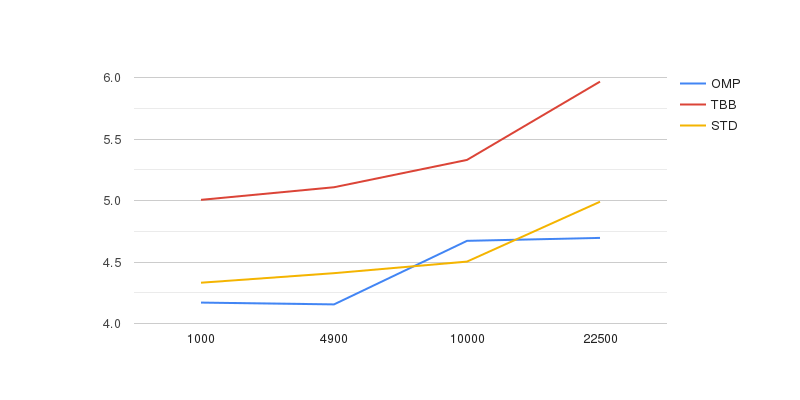
\includegraphics[width=1\textwidth]{chart(5).png}
\caption{\label{fig:График}График ускорения вычислений}
\end{figure}
\par В данной лабораторной работе наилучшее ускорение получилось добиться при использовании технологии TBB. Данный инструмент использует максимальные возможности системы благодаря своей архитектуре. Из полученных данных, можно сделать вывод, что улучшение производительности заметнее всего на матрицах, чей размер достаточно велик. Небольшие матрицы не могут дать высоко коэффициента ускорения.
\newpage
\section*{Заключение}
\addcontentsline{toc}{section}{Заключение}
\par В ходе данной лабораторной работы было реализовано умножение разреженных матриц в формате CRS. Итоговое приложение было разделено на три вида: использование технологии OMP, TBB и STD для распределения вычислений между потоками. Для проверки работы алгоритмов были написаны тестовые случаи с использованием Google C++ Testing Framework. Заключительные эксперименты показали эффективность работы полученных алгоритмов.
\newpage
\section*{Литература}
\addcontentsline{toc}{section}{Литература}
\begin{itemize}
\item Гергель В.П., Стронгин Р.Г. Основы параллельных вычислений для многопроцессорных вычислительных систем. Учебное пособие – Нижний Новгород: Изд-во ННГУ им. Н.И. Лобачевского, 2003. 184 с. ISBN 5-85746-602-4.
\item Баркалов К.А. Параллельные численные методы. Решение разреженных СЛАУ. Н. Новгород: Изд-во Нижегородского госуниверситета им. Н.И. Лобачевского, 2011
\end{itemize}
\newpage
\section*{Приложение}
\addcontentsline{toc}{section}{Приложение}
\subsection*{Вспомагатиельные функции}
\addcontentsline{toc}{subsection}{Вспомагатиельные функции}
\begin{lstlisting}
//=======================================================================
// function : TransformToNorm
// purpose  :
//=======================================================================

std::vector<std::complex<double>> TransformToNorm(const Matrix& A) {
  std::vector<std::complex<double>> Res(A.Lenght * A.Lenght, 0.);
  for (size_t i = 0; i < A.Lenght; ++i) {
    const size_t i1 = A.RowInd.at(i);
    const size_t i2 = A.RowInd.at(i + 1) - 1;
    for (size_t j = i1; j <= i2; j++) {
      Res.at(i * A.Lenght + A.Column.at(j)) = A.Values.at(j);
    }
  }
  return Res;
}

//=======================================================================
// function : GenerateCRS
// purpose  :
//=======================================================================

Matrix GenerateCRS(const size_t lenght) {
  Matrix Res;
  if (lenght < 1) {
    return Res;
  }

  std::mt19937 generator(static_cast<unsigned int>(time(0)));
  size_t ValueInRow = (lenght > 1) ? 1 + generator() % (lenght / 2) : 1;
  size_t VCount = ValueInRow * lenght;

  Res.Lenght = lenght;
  Res.VCount = VCount;
  Res.RowInd = std::vector<size_t>(lenght + 1);
  Res.Column = std::vector<size_t>(VCount);
  Res.Values = std::vector<std::complex<double>>(VCount);

  for (size_t i = 0; i < lenght; i++) {
    for (size_t j = 0; j < ValueInRow; j++) {
      bool isValue = false;
      do {
        isValue = false;
        Res.Column.at(i * ValueInRow + j) =
            (lenght > 1) ? 1 + generator() % (lenght - 1) : 0;
        for (size_t k = 0; k < j; k++) {
          if (Res.Column.at(i * ValueInRow + j) ==
              Res.Column.at(i * ValueInRow + k)) {
            isValue = true;
          }
        }
      } while (isValue);
    }
    for (size_t j = 0; j < ValueInRow - 1; j++) {
      for (size_t k = 0; k < ValueInRow - 1; k++) {
        if (Res.Column.at(i * ValueInRow + k) >
            Res.Column.at(i * ValueInRow + k + 1)) {
          std::swap(Res.Column.at(i * ValueInRow + k),
                    Res.Column.at(i * ValueInRow + k + 1));
        }
      }
    }
  }

  for (auto& iter : Res.Values) {
    iter = std::complex<double>(generator() % 110, generator() % 110);
  }

  size_t Count = 0;
  for (auto& iter : Res.RowInd) {
    iter = Count;
    Count += ValueInRow;
  }

  return Res;
}

//=======================================================================
// function : MultNorm
// purpose  :
//=======================================================================

std::vector<std::complex<double>> MultNorm(
    const std::vector<std::complex<double>>& A,
    const std::vector<std::complex<double>>& B, const size_t lenght) {
  std::vector<std::complex<double>> Res(A.size());
  for (size_t i = 0; i < lenght; i++) {
    for (size_t j = 0; j < lenght; j++) {
      std::complex<double> sum = 0;
      for (size_t k = 0; k < lenght; k++) {
        sum += A.at(i * lenght + k) * B.at(k * lenght + j);
      }
      Res.at(i * lenght + j) = sum;
    }
  }
  return Res;
}

//=======================================================================
// function : CompareCRS
// purpose  :
//=======================================================================

bool Compare_Vector(const std::vector<size_t>& A,
                    const std::vector<size_t>& B) {
  for (size_t i = 0; i < A.size(); i++) {
    if (A.at(i) != B.at(i)) {
      return false;
    }
  }
  return true;
}

bool Compare_Vector(const std::vector<std::complex<double>>& A,
                    const std::vector<std::complex<double>>& B) {
  for (size_t i = 0; i < A.size(); i++) {
    if (abs(A.at(i) - B.at(i)) > 1e-8) {
      return false;
    }
  }
  return true;
}

bool CompareCRS(const Matrix& A, const Matrix& B) {
  if (A.Lenght != B.Lenght || A.VCount != B.VCount ||
      !Compare_Vector(A.Column, B.Column) ||
      !Compare_Vector(A.Values, B.Values) ||
      !Compare_Vector(A.RowInd, B.RowInd)) {
    return false;
  }
  return true;
}
\end{lstlisting}
\newpage
\subsection*{Последотовательный алгоритм}
\addcontentsline{toc}{subsection}{Последотовательный алгоритм}
\begin{lstlisting}
//=======================================================================
// function : MultCRS
// purpose  :
//=======================================================================

Matrix MultCRS(const Matrix& A, const Matrix& b) {
  const size_t N = A.Lenght;
  const size_t N2 = b.Lenght;
  Matrix Res, B;

  B.Lenght = b.Lenght;
  B.VCount = b.VCount;
  B.Column = std::vector<size_t>(b.VCount);
  B.RowInd = std::vector<size_t>(b.Lenght + 1);
  B.Values = std::vector<std::complex<double>>(b.VCount);

  for (const auto& iter : b.Column) {
    B.RowInd.at(iter + 1)++;
  }

  size_t Index_tmp = 0;
  for (auto& iter : B.RowInd) {
    const size_t tmp = iter;
    iter = Index_tmp;
    Index_tmp = Index_tmp + tmp;
  }

  for (size_t i = 0; i < b.Lenght; i++) {
    size_t j1 = b.RowInd.at(i);
    size_t j2 = b.RowInd.at(i + 1);
    size_t Col = i;
    for (size_t j = j1; j < j2; j++) {
      std::complex<double> V = b.Values.at(j);
      size_t Row_index = b.Column.at(j);
      size_t IIndex = B.RowInd.at(Row_index + 1);
      B.Values.at(IIndex) = V;
      B.Column.at(IIndex) = Col;
      B.RowInd.at(Row_index + 1)++;
    }
  }

  Res.Lenght = N;
  Res.RowInd.push_back(0);
  for (size_t i = 0; i < N; i++) {
    size_t rowNZ = 0;
    for (size_t j = 0; j < N2; j++) {
      std::complex<double> sum = 0;
      for (size_t k = A.RowInd.at(i); k < A.RowInd.at(i + 1); k++) {
        for (size_t l = B.RowInd.at(j); l < B.RowInd.at(j + 1); l++) {
          if (A.Column.at(k) == B.Column.at(l)) {
            sum += A.Values.at(k) * B.Values.at(l);
            break;
          }
        }
      }

      if (abs(sum) > std::numeric_limits<double>::epsilon()) {
        Res.Column.push_back(j);
        Res.Values.push_back(sum);
        rowNZ++;
      }
    }
    Res.RowInd.push_back(rowNZ + Res.RowInd.at(i));
  }
  Res.VCount = Res.Column.size();
  return Res;
}
\end{lstlisting}
\newpage
\subsection*{Алгоритм OMP}
\addcontentsline{toc}{subsection}{Алгоритм OMP}
\begin{lstlisting}
//=======================================================================
// function : MultCRS_OMP
// purpose  :
//=======================================================================

Matrix MultCRS_OMP(const Matrix& A, const Matrix& b) {
  const size_t N = A.Lenght;
  const size_t N2 = b.Lenght;
  const int size = static_cast<int>(b.VCount);
  Matrix Res, B;

  B.Lenght = N2;
  B.VCount = N2;
  B.Column = std::vector<size_t>(b.VCount);
  B.RowInd = std::vector<size_t>(N2 + 2);
  B.Values = std::vector<std::complex<double>>(b.VCount);

  for (int i = 0; i < size; i++) {
    ++B.RowInd.at(b.Column.at(i) + 2);
  }

#pragma omp parallel for ordered
  for (int i = 2; i < static_cast<int>(N2) + 2; i++) {
#pragma omp ordered
    B.RowInd.at(i) += B.RowInd.at(i - 1);
  }

#pragma omp parallel for
  for (int i = 0; i < static_cast<int>(N2); ++i) {
    const int end = static_cast<int>(b.RowInd.at(i + 1));
    for (int j = static_cast<int>(b.RowInd.at(i)); j < end; ++j) {
      {
        const size_t old_index = b.Column.at(j) + 1;
        size_t new_index = 0;
#pragma omp critical
        {
          new_index = B.RowInd.at(old_index);
          B.RowInd.at(old_index)++;
        }
        B.Values.at(new_index) = b.Values.at(j);
        B.Column.at(new_index) = i;
      }
    }
  }
  B.RowInd.pop_back();

  Res.Lenght = N;
  Res.RowInd = std::vector<size_t>(N2 + 1);
  std::vector<std::pair<size_t, std::complex<double>>> aColCalues(N * N);

#pragma omp parallel for
  for (int i = 0; i < static_cast<int>(N); i++) {
    size_t rowNZ = 0;
    for (size_t j = 0; j < N2; j++) {
      std::complex<double> sum = 0;
      size_t end_k = A.RowInd.at(i + 1);
      size_t end_l = B.RowInd.at(j + 1);
      for (size_t k = A.RowInd.at(i); k < end_k; k++) {
        for (size_t l = B.RowInd.at(j); l < end_l; l++) {
          if (A.Column.at(k) == B.Column.at(l)) {
            sum += A.Values.at(k) * B.Values.at(l);
            break;
          }
        }
      }

      if (abs(sum) > 1e-8) {
        std::pair<size_t, std::complex<double>> aPair{j, sum};
        std::swap(aColCalues.at(i * N + rowNZ), aPair);
        rowNZ++;
      }
    }
    Res.RowInd.at(i + 1) = rowNZ;
  }
#pragma omp parallel for ordered
  for (int i = 1; i < static_cast<int>(N2) + 1; i++) {
#pragma omp ordered
    Res.RowInd.at(i) += Res.RowInd.at(i - 1);
  }
  const size_t res_size = Res.RowInd.back();
  Res.Column = std::vector<size_t>(res_size);
  Res.Values = std::vector<std::complex<double>>(res_size);
#pragma omp parallel for
  for (int i = 0; i < static_cast<int>(N); i++) {
    const size_t start_ind = Res.RowInd.at(i);
    const size_t end_ind = Res.RowInd.at(i + 1);
    size_t own_ind = 0;
    for (size_t j = start_ind; j < end_ind; j++, own_ind++) {
      const std::pair<size_t, std::complex<double>> aPair(
          std::move(aColCalues.at(i * N + own_ind)));
      Res.Column.at(j) = aPair.first;
      Res.Values.at(j) = aPair.second;
    }
  }
  Res.VCount = Res.Column.size();
  return Res;
}
\end{lstlisting}

\newpage
\subsection*{Алгоритм TBB}
\addcontentsline{toc}{subsection}{Алгоритм TBB}
\begin{lstlisting}
//=======================================================================
// function : MultCRS_TBB
// purpose  :
//=======================================================================

Matrix MultCRS_TBB(const Matrix& A, const Matrix& b) {
  const size_t N = A.Lenght;
  const size_t N2 = b.Lenght;
  const size_t size = b.VCount;
  Matrix Res, B;

  B.Lenght = N2;
  B.VCount = N2;
  B.Column = std::vector<size_t>(b.VCount);
  B.RowInd = std::vector<size_t>(N2 + 2);
  B.Values = std::vector<std::complex<double>>(b.VCount);

  for (size_t i = 0; i < size; i++) {
    ++B.RowInd.at(b.Column.at(i) + 2);
  }

  for (size_t i = 2; i < N2 + 2; i++) {
    B.RowInd.at(i) += B.RowInd.at(i - 1);
  }

  tbb::task_scheduler_init init;
  tbb::mutex aMutex;
  tbb::parallel_for(tbb::blocked_range<size_t>(0, N2, 10),
                    [&](const tbb::blocked_range<size_t>& r) {
                      for (size_t i = r.begin(); i < r.end(); ++i) {
                        const size_t end = b.RowInd.at(i + 1);
                        for (size_t j = b.RowInd.at(i); j < end; ++j) {
                          {
                            const size_t old_index = b.Column.at(j) + 1;
                            size_t new_index = 0;
                            aMutex.lock();
                            new_index = B.RowInd.at(old_index);
                            B.RowInd.at(old_index)++;
                            aMutex.unlock();
                            B.Values.at(new_index) = b.Values.at(j);
                            B.Column.at(new_index) = i;
                          }
                        }
                      }
                    });
  B.RowInd.pop_back();

  Res.Lenght = N;
  Res.RowInd = std::vector<size_t>(N2 + 1);
  std::vector<std::pair<size_t, std::complex<double>>> aColCalues(N * N);
  tbb::parallel_for(
      tbb::blocked_range<size_t>(0, N, 10),
      [&](const tbb::blocked_range<size_t>& r) {
        for (size_t i = r.begin(); i < r.end(); i++) {
          size_t rowNZ = 0;
          for (size_t j = 0; j < N2; j++) {
            std::complex<double> sum = 0;
            size_t end_k = A.RowInd.at(i + 1);
            size_t end_l = B.RowInd.at(j + 1);
            for (size_t k = A.RowInd.at(i); k < end_k; k++) {
              for (size_t l = B.RowInd.at(j); l < end_l; l++) {
                if (A.Column.at(k) == B.Column.at(l)) {
                  sum += A.Values.at(k) * B.Values.at(l);
                  break;
                }
              }
            }

            if (abs(sum) > 1e-8) {
              std::pair<size_t, std::complex<double>> aPair{j, sum};
              std::swap(aColCalues.at(i * N + rowNZ), aPair);
              rowNZ++;
            }
          }
          Res.RowInd.at(i + 1) = rowNZ;
        }
      });

  for (size_t i = 1; i < N2 + 1; i++) {
    Res.RowInd.at(i) += Res.RowInd.at(i - 1);
  }

  const size_t res_size = Res.RowInd.back();
  Res.Column = std::vector<size_t>(res_size);
  Res.Values = std::vector<std::complex<double>>(res_size);
  tbb::parallel_for(tbb::blocked_range<size_t>(0, N, 10),
                    [&](const tbb::blocked_range<size_t>& r) {
                      for (size_t i = r.begin(); i < r.end(); i++) {
                        const size_t start_ind = Res.RowInd.at(i);
                        const size_t end_ind = Res.RowInd.at(i + 1);
                        size_t own_ind = 0;
                        for (size_t j = start_ind; j < end_ind;
                             j++, own_ind++) {
                          const std::pair<size_t, std::complex<double>> aPair(
                              std::move(aColCalues.at(i * N + own_ind)));
                          Res.Column.at(j) = aPair.first;
                          Res.Values.at(j) = aPair.second;
                        }
                      }
                    });
  init.terminate();
  Res.VCount = Res.Column.size();
  return Res;
}
\end{lstlisting}


\newpage
\subsection*{Алгоритм STD}
\addcontentsline{toc}{subsection}{Алгоритм STD}
\begin{lstlisting}
//=======================================================================
// function : MultCRS_STD
// purpose  :
//=======================================================================

std::mutex g_lock;

Matrix MultCRS_STD(const Matrix& A, const Matrix& b) {
  const size_t NbThreads = std::thread::hardware_concurrency();
  const size_t N = A.Lenght;
  const size_t N2 = b.Lenght;
  const size_t size = b.VCount;
  Matrix Res, B;

  B.Lenght = N2;
  B.VCount = N2;
  B.Column = std::vector<size_t>(b.VCount);
  B.RowInd = std::vector<size_t>(N2 + 2);
  B.Values = std::vector<std::complex<double>>(b.VCount);

  for (size_t i = 0; i < size; i++) {
    ++B.RowInd.at(b.Column.at(i) + 2);
  }

  for (size_t i = 2; i < N2 + 2; i++) {
    B.RowInd.at(i) += B.RowInd.at(i - 1);
  }

  {
    std::vector<std::thread> threads(NbThreads);
    auto tranport = [&](const size_t start, const size_t end) {
      for (size_t i = start; i < end; ++i) {
        const size_t end = b.RowInd.at(i + 1);
        for (size_t j = b.RowInd.at(i); j < end; ++j) {
          {
            const size_t old_index = b.Column.at(j) + 1;
            size_t new_index = 0;
            {
              std::lock_guard<std::mutex> anObj(g_lock);
              new_index = B.RowInd.at(old_index);
              B.RowInd.at(old_index)++;
            }
            B.Values.at(new_index) = b.Values.at(j);
            B.Column.at(new_index) = i;
          }
        }
      }
    };
    const size_t for_thread = N2 / NbThreads;
    size_t count = 0;
    for (size_t i = 0; i < NbThreads - 1; i++) {
      const size_t end = count + for_thread;
      threads.at(i) = std::thread(tranport, count, end);
      count += for_thread;
    }
    threads.back() = std::thread(tranport, count, N2);

    for (auto& it : threads) {
      it.join();
    }
  }

  B.RowInd.pop_back();

  Res.Lenght = N;
  Res.RowInd = std::vector<size_t>(N2 + 1);
  std::vector<std::pair<size_t, std::complex<double>>> aColCalues(N * N);

  {
    std::vector<std::thread> threads(NbThreads);
    auto mult = [&](const size_t start, const size_t end) {
      for (size_t i = start; i < end; ++i) {
        size_t rowNZ = 0;
        for (size_t j = 0; j < N2; j++) {
          std::complex<double> sum = 0;
          size_t end_k = A.RowInd.at(i + 1);
          size_t end_l = B.RowInd.at(j + 1);
          for (size_t k = A.RowInd.at(i); k < end_k; k++) {
            for (size_t l = B.RowInd.at(j); l < end_l; l++) {
              if (A.Column.at(k) == B.Column.at(l)) {
                sum += A.Values.at(k) * B.Values.at(l);
                break;
              }
            }
          }

          if (abs(sum) > 1e-8) {
            std::pair<size_t, std::complex<double>> aPair{j, sum};
            std::swap(aColCalues.at(i * N + rowNZ), aPair);
            rowNZ++;
          }
        }
        Res.RowInd.at(i + 1) = rowNZ;
      }
    };
    const size_t for_thread = N / NbThreads;
    size_t count = 0;
    for (size_t i = 0; i < NbThreads - 1; i++) {
      const size_t end = count + for_thread;
      threads.at(i) = std::thread(mult, count, end);
      count += for_thread;
    }
    threads.back() = std::thread(mult, count, N);

    for (auto& it : threads) {
      it.join();
    }
  }

  for (size_t i = 1; i < N2 + 1; i++) {
    Res.RowInd.at(i) += Res.RowInd.at(i - 1);
  }

  const size_t res_size = Res.RowInd.back();
  Res.Column = std::vector<size_t>(res_size);
  Res.Values = std::vector<std::complex<double>>(res_size);

  {
    std::vector<std::thread> threads(NbThreads);
    auto filling = [&](const size_t start, const size_t end) {
      for (size_t i = start; i < end; ++i) {
        const size_t start_ind = Res.RowInd.at(i);
        const size_t end_ind = Res.RowInd.at(i + 1);
        size_t own_ind = 0;
        for (size_t j = start_ind; j < end_ind; j++, own_ind++) {
          const std::pair<size_t, std::complex<double>> aPair(
              std::move(aColCalues.at(i * N + own_ind)));
          Res.Column.at(j) = aPair.first;
          Res.Values.at(j) = aPair.second;
        }
      }
    };
    const size_t for_thread = N / NbThreads;
    size_t count = 0;
    for (size_t i = 0; i < NbThreads - 1; i++) {
      const size_t end = count + for_thread;
      threads.at(i) = std::thread(filling, count, end);
      count += for_thread;
    }
    threads.back() = std::thread(filling, count, N);

    for (auto& it : threads) {
      it.join();
    }
  }
  Res.VCount = Res.Column.size();
  return Res;
}
\end{lstlisting}



\end{document}